% Guia de estudo — tese curta (PT-PT).
% NÃO é um resumo da tese: ENSINA, do zero, o que é preciso para a defender.
% O Nível 0 existe porque o autor disse, com razão, que não tinha as bases de IA.

\documentclass[aspectratio=169]{beamer}
\usetheme{Madrid}
\usecolortheme{dolphin}
\usepackage[T1]{fontenc}
\usepackage[portuguese,shorthands=off]{babel}
\usepackage{booktabs}
\usepackage{tikz}
\usetikzlibrary{positioning, arrows.meta, calc, decorations.pathreplacing}
\tikzset{every node/.append style={execute at begin node={\hyphenpenalty=10000\exhyphenpenalty=10000\relax}}}
% As figuras vem da arvore CANONICA. Antes vinham de ../figures (a arvore antiga, de
% onde estes materiais foram movidos) e de ../../thesis, que foi arquivada. Sem isto o
% LaTeX compila em modo rascunho, o numero de paginas nao muda, e o PDF sai SEM AS
% IMAGENS -- que e um defeito que a contagem de paginas esconde.
\graphicspath{{../figures/}}
\usepackage{xcolor}
% A marca: o verde de `app/assets/logo.svg`, e o "G" e o trocadilho inteiro --
% inveSTIGATE + alliGATOR. Uma macro so, para o nome nunca sair escrito de duas
% maneiras diferentes em dois sitios.
\definecolor{marca}{HTML}{0A8F52}
\newcommand{\gator}{Investi\textcolor{marca}{G}ator}
\setbeamertemplate{navigation symbols}{}
\newcommand{\key}[1]{\textbf{\textcolor{blue!55!black}{#1}}}

\title[Guia de estudo]{Guia de estudo do \gator}
\titlegraphic{
\includegraphics[height=0.95cm]{logo_lockup.png}}
\subtitle{Do zero até conseguir defender}
\author{Henrique J.\ S.\ Santos}
\date{}

\begin{document}

\begin{frame}\titlepage\end{frame}

\begin{frame}{Como usar este guia}
\begin{itemize}
  \item \key{Nível 0}: as bases de IA. Só o que esta tese usa, nada mais.
  \item \key{Nível 1}: o problema e o sistema.
  \item \key{Níveis 2 a 4}: uma técnica de cada vez, com contas feitas.
  \item \key{Nível 5}: os números que tens de saber de cor.
  \item \key{Nível 6}: as perguntas do júri, com resposta.
\end{itemize}
\vspace{4mm}
\begin{center}
Se só tiveres uma hora: \key{Nível 5} e \key{Nível 6}.\\
Se tiveres uma tarde: tudo, por ordem.
\end{center}
\end{frame}

% ═══════════════ NÍVEL 0 ═══════════════
\begin{frame}{\key{Nível 0}: IA, aprendizagem automática, e o que tu usas}
\begin{itemize}
  \item \key{Inteligência artificial} é o guarda-chuva: qualquer sistema que faça algo que
        associamos a inteligência.
  \item \key{Aprendizagem automática (ML)} é um pedaço desse guarda-chuva: em vez de escreveres a
        regra, dás \textbf{exemplos} e o programa encontra a regra.
  \item \key{Aprendizagem profunda} é um pedaço do ML: redes neuronais com muitas camadas.
\end{itemize}
\vspace{4mm}
\begin{block}{Na tua tese}
Usas \textbf{estatística} nas técnicas 1 e 2 (o \emph{z}-score e a decomposição do movimento),
\textbf{aprendizagem profunda já treinada por outros} na técnica 3 (os \emph{embeddings} de frase)
e \textbf{aprendizagem automática treinada por ti} na técnica 4 (a triagem).\\
\textbf{Não} treinas redes neuronais. \textbf{Não} usas visão computacional. \textbf{Não} usas
aprendizagem por reforço. Diz isso sem hesitar.
\end{block}
\end{frame}

\begin{frame}{\key{Nível 0}: as palavras que vais ouvir}
\small
\begin{tabular}{p{0.24\textwidth} p{0.68\textwidth}}
\toprule
\key{Features} & As colunas que o modelo vê. \textbf{Na tese escreves «entradas»}: se ouvires
\emph{features}, é disto que falam. Na tua: volatilidade, momento, movimento do dia,
comprimento do título, setor. \\
\key{Rótulo} & A resposta certa, conhecida. Na tua: houve movimento anormal a seguir? Sim/não. \\
\key{Treino / teste} & Ensinas com uns dados, avalias com \emph{outros}. Se avaliasses com os
mesmos, media memória e não aprendizagem. \\
\key{Linha de base} & O método simples contra o qual comparas. Sem ele, um número não quer dizer
nada. \\
\key{Sobreajuste} & O modelo decora o treino e falha no resto. É o que a divisão treino/teste
deteta. \\
\key{Calibração} & Fazer com que ``70\%'' queira mesmo dizer 70\% das vezes. \\
\bottomrule
\end{tabular}
\end{frame}

\begin{frame}{\key{Nível 0}: a pergunta que te vão fazer e a resposta}
\begin{center}
\emph{``Isto aprende sozinho? Melhora com o tempo?''}
\end{center}
\vspace{4mm}
\begin{block}{Resposta}
\textbf{Não.} O modelo foi treinado uma vez, sobre dados de 2018--2023, e está \key{congelado}.\\
Quando corre em produção faz \key{inferência}, ou seja, aplica o que aprendeu, e \textbf{não} volta a
aprender.
\end{block}
\vspace{3mm}
\footnotesize
Três coisas diferentes que é fácil confundir:\\
\key{treino} (aprender dos exemplos, uma vez) $\neq$
\key{inferência} (aplicar, todos os dias) $\neq$
\key{re-treino} (voltar a treinar com dados novos, o que não é feito).
\end{frame}

% ═══════════════ NÍVEL 1 ═══════════════
\begin{frame}{\key{Nível 1}: as três perguntas}
\begin{enumerate}
  \item \key{Isto é invulgar?} estatística
  \item \key{Foi a empresa ou o mercado?} decomposição
  \item \key{Já aconteceu, e o que se seguiu?} recuperação e medição
\end{enumerate}
\vspace{4mm}
\begin{block}{Guarda esta frase}
``As aplicações gratuitas mostram a percentagem, que é o \emph{princípio} da primeira pergunta e não
a resposta. Os terminais profissionais respondem às três e não estão ao alcance deste
investidor. Se te perguntarem quanto custam, a resposta é que o preço não é publicado de
forma citável, e é a indisponibilidade que sustenta o argumento, não um valor concreto.
\textbf{O problema não é científico, é de acesso.}''
\end{block}
\end{frame}

\begin{frame}{\key{Nível 1}: o que o sistema recusa fazer}
\begin{center}
\Large Não prevê preços. Não aconselha. Não gere carteiras.
\end{center}
\vspace{5mm}
\begin{block}{Porque é que isto é uma força}
Uma afirmação sobre o que \textbf{já aconteceu} confere-se contra o registo.\\
Uma previsão só se confere depois de já ter sido preciso decidir.\\[2mm]
E há uma razão teórica: se o futuro fosse previsível a partir de informação \emph{pública}, essa
informação já estaria no preço.
\end{block}
\end{frame}

% ═══════════════ NÍVEL 2 ═══════════════
% O produto, capturado da producao. Esta aqui porque o aluno estuda por este ficheiro e tem de
% conseguir apontar para o ecra e dizer o que cada parte responde.
\begin{frame}{\key{Nível 1}: e é isto que está no ar}
\begin{columns}[T]
\begin{column}{0.60\textwidth}
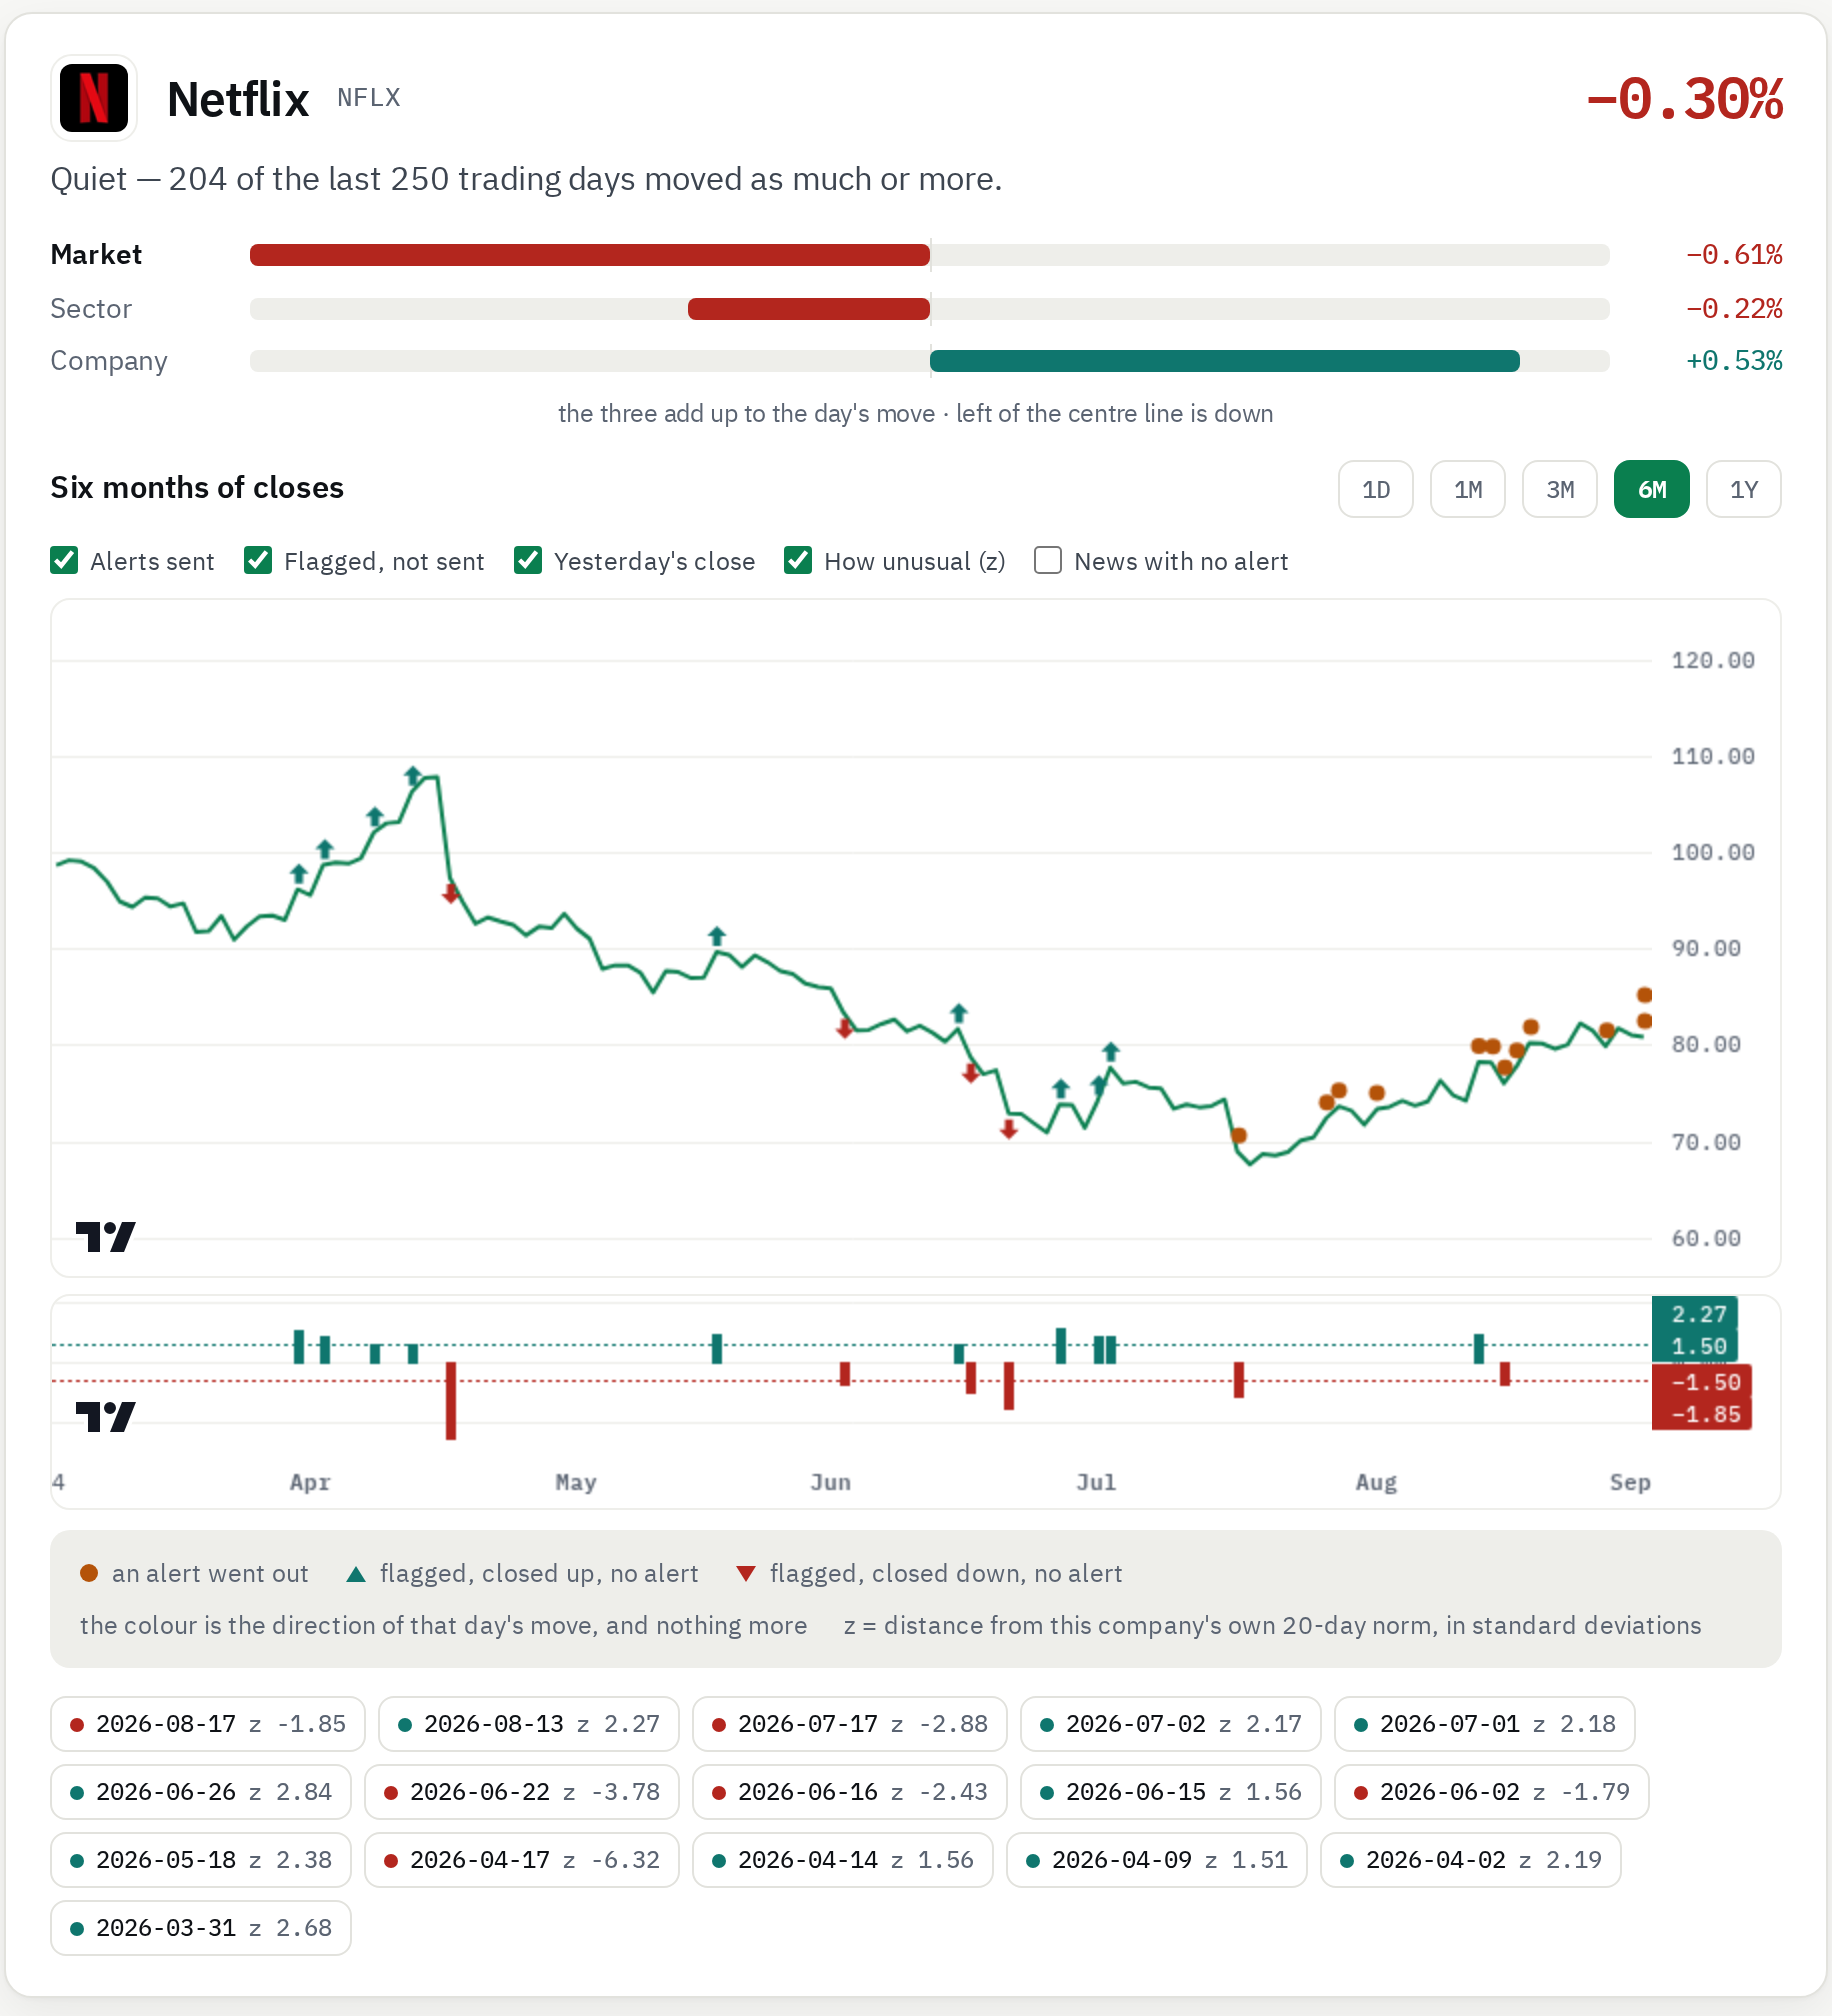
\includegraphics[width=\textwidth,height=0.78\textheight,keepaspectratio]{app_v7_empresa.png}
\end{column}
\begin{column}{0.37\textwidth}
\small
Captura real da produção, com a sessão a decorrer.
\vspace{2mm}
\begin{itemize}
  \item A \key{frase} vem antes do número: é a regra de apresentação.
  \item A \key{repartição} responde à segunda pergunta. Aqui a ação desce $0{,}30\%$,
        mas a contribuição da própria empresa é \textbf{positiva}: quem a puxa é o \textbf{mercado}.
  \item Os \key{marcadores} na curva separam os dias que deram alerta dos que o
        detetor assinalou e não deram. A distância entre uns e outros é o custo das portas.
\end{itemize}
\end{column}
\end{columns}
\end{frame}

\begin{frame}{\key{Nível 1}: e o que nenhum produto mostra}
A mesma página abre, para cada candidata, \key{o percurso pelas portas} e onde parou.
\vspace{2mm}
\begin{center}
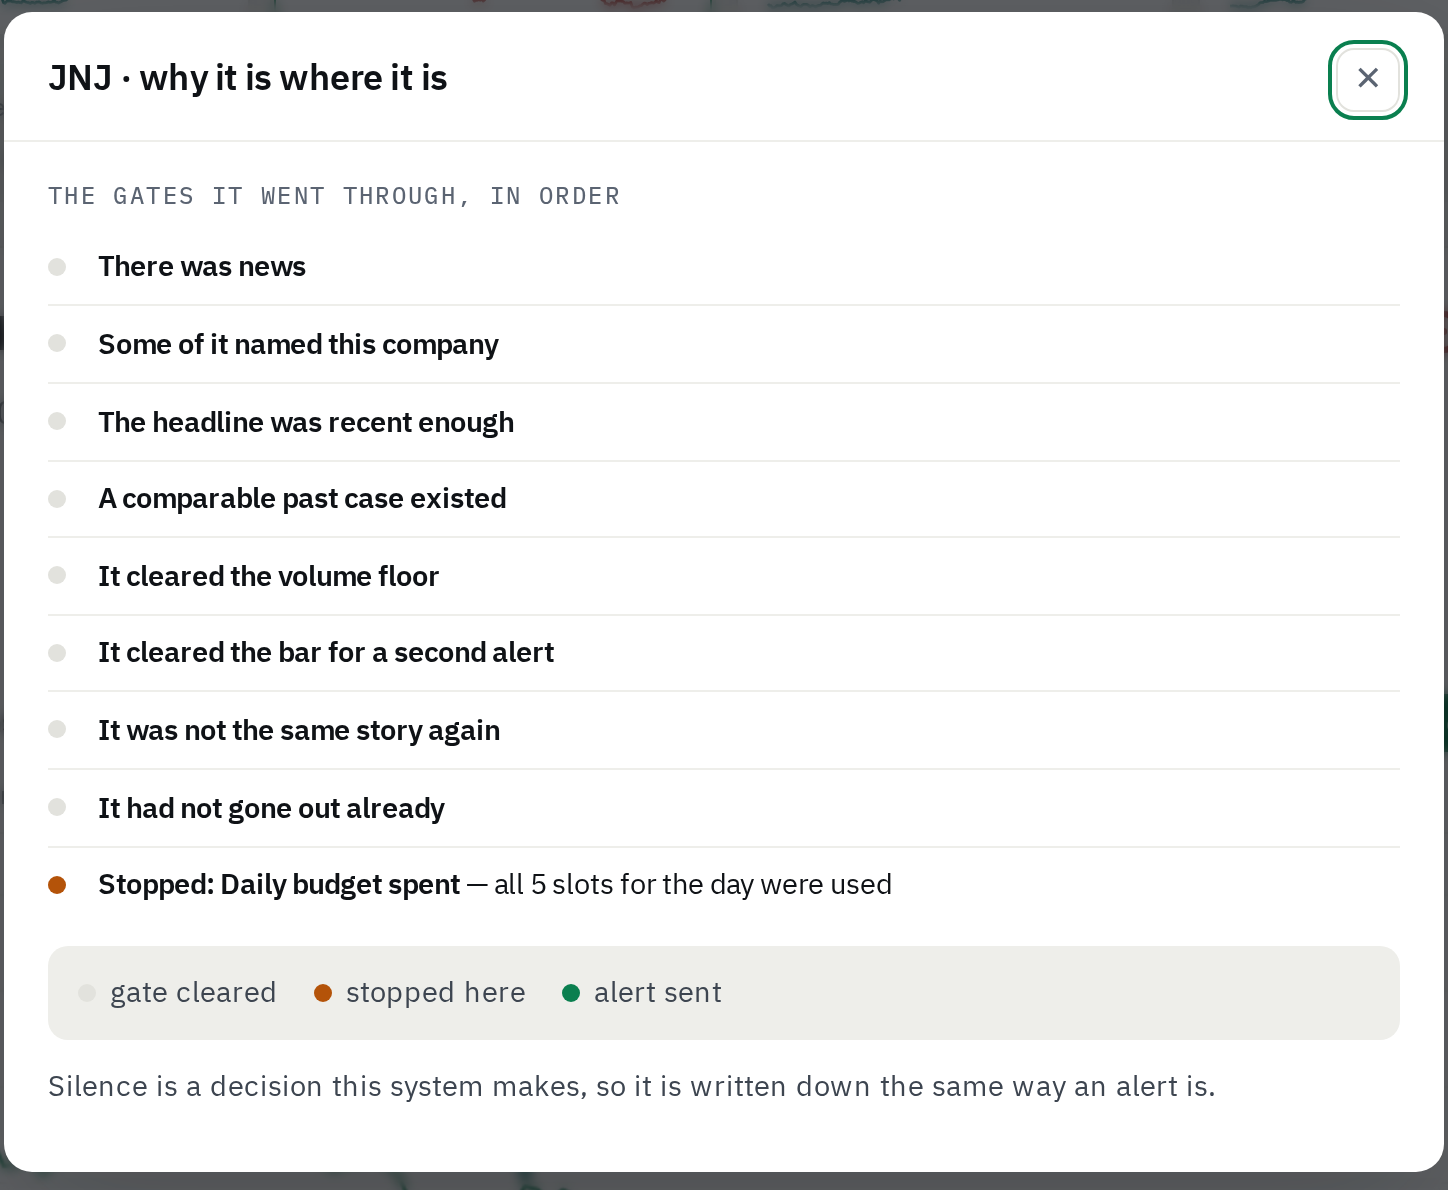
\includegraphics[width=0.95\textwidth,height=0.55\textheight,keepaspectratio]{app_v7_silencio.png}
\end{center}
\vspace{1mm}
{\footnotesize Se te perguntarem \emph{``e quando não envia nada?''}, é para aqui que
apontas: nove em cada dez varreduras não enviam, e cada etapa diz a porta que a deteve
(aqui, o orçamento de cinco alertas do dia, já gasto).}
\end{frame}

\begin{frame}{\key{Nível 2}, técnica 1: o \emph{z}-score, com contas}
\begin{center}
$z = \dfrac{\text{movimento de hoje} - \text{média dos 20 dias}}{\text{desvio-padrão dos 20 dias}}$
\end{center}
\vspace{3mm}
\small
Exemplo real (Tesla, 24 out 2024):
\begin{center}
\begin{tabular}{lr}
\toprule
Média dos 20 dias anteriores & $-0{,}92\%$ \\
Desvio-padrão desses 20 dias & $2{,}725\%$ \\
Movimento do dia & $+19{,}82\%$ \\
\midrule
$z = (19{,}82 - (-0{,}92)) / 2{,}725$ & $\mathbf{+7{,}61}$ \\
\bottomrule
\end{tabular}
\end{center}
\vspace{2mm}
\footnotesize
\key{Faz esta conta à mão uma vez.} Se te pedirem para a explicar no quadro, tens de a saber fazer.
\end{frame}

\begin{frame}{\key{Nível 2}: a parte que te vão testar}
\begin{center}
\emph{``Porque é que o dia de hoje não entra no cálculo da sua própria norma?''}
\end{center}
\vspace{4mm}
\begin{block}{Resposta}
Porque se entrasse, um dia extremo puxava a média e aumentava o desvio-padrão, e ficaria a
parecer \textbf{menos} invulgar do que foi.\\[2mm]
Isso seria usar informação que, no momento da decisão, ainda não devia contar. Chama-se
\key{lookahead}, e é o erro mais comum em modelos financeiros.
\end{block}
\vspace{2mm}
\footnotesize
Na tese isto é garantido por \textbf{um teste automático}, não por uma promessa: o teste altera o
futuro e exige que as \emph{features} fiquem iguais e o rótulo mude.
\par\smallskip
\textbf{Caso limite:} se os vinte dias forem constantes, manter o mesmo valor não dispara; um salto
dispara com a explicação \emph{``norma plana; $z$ indefinido''}. Nunca digas que esse salto tem
$z=0$.
\end{frame}

\begin{frame}{\key{Nível 2}, técnica 2: foi a empresa, ou foi o mercado?}
\small
Responde à \key{segunda} das três perguntas, e é a que um arguente com finanças conhece.
\vspace{2mm}
\begin{itemize}
  \item \key{A conta:} o movimento do dia parte-se em três parcelas que \textbf{somam ao}
        \textbf{total}: \emph{mercado} (o beta vezes o índice), \emph{setor} (o fundo do setor,
        já descontado do mercado) e \emph{empresa} (o que sobra).
  \item \key{Os betas} são estimados só com dias \textbf{anteriores} ao dia explicado, e
        \textbf{encolhidos} pela sua precisão: mercado para $1$, setor ortogonalizado para $0$
        (Vasicek, 1973). O desvio-padrão comum do prior é $0{,}5$.
  \item \key{Porquê encolher:} sem isso, um beta mal estimado atribuía o movimento inteiro à
        empresa.
\end{itemize}
\vspace{2mm}
\begin{block}{O que dizes se te perguntarem se está certa}
``As parcelas somam sempre, por construção, portanto isso não prova nada. Medi as duas coisas
que podiam falhar: se a repartição \textbf{discrimina} (num mesmo dia o motor foi a empresa em
$8$ casos, o mercado em $5$ e o setor em $4$, logo não diz sempre o mesmo) e se os
\textbf{betas} estão bem estimados ($R^2$ mediano $0{,}460$, e \textbf{numa das dezassete foi}
\textbf{negativo}). E não há verdade humana para comparar: é por isso que esta
técnica não dá origem a uma pergunta de investigação.''
\end{block}
\end{frame}

% ═══════════════ NÍVEL 3 ═══════════════
\begin{frame}{\key{Nível 3}, técnica 3: frases como pontos}
\begin{itemize}
  \item Um \key{embedding} é uma lista de números que representa uma frase: aqui, \textbf{384}.
  \item Funciona como uma \textbf{coordenada de significado}: frases parecidas ficam perto.
  \item Compara-se pelo \key{cosseno}: o \textbf{ângulo} entre duas direções, entre $-1$ e $1$.
\end{itemize}
\vspace{3mm}
\begin{block}{Porquê o ângulo e não a distância?}
Porque interessa \emph{sobre o que} a frase fala, não o comprimento do texto. Um título curto e
um parágrafo longo sobre o mesmo assunto devem ficar próximos.
\end{block}
\vspace{2mm}
\footnotesize
\key{O modelo não é teu}: é pré-treinado (Sentence-BERT). Diz isso; está declarado na tese.
\end{frame}

\begin{frame}{\key{Nível 3}: tema não é direção}
\begin{center}
\large É a ressalva mais importante desta técnica.
\end{center}
\vspace{4mm}
Duas notícias podem ser sobre \textbf{o mesmo assunto} e o preço ter ido para \textbf{lados
opostos}.
\vspace{3mm}
\begin{block}{Medido}
Concordância de direção entre a notícia e os casos recuperados: \key{0{,}708}\\
Chão de acaso: \key{0{,}688}\\[2mm]
Ou seja: \textbf{quase nada}.
\end{block}
\vspace{2mm}
\footnotesize
É por isso que o sistema mostra os casos \textbf{um a um} e nunca só a média. Uma média
esconderia que foram em sentidos opostos.
\end{frame}

% ═══════════════ NÍVEL 4 ═══════════════
\begin{frame}{\key{Nível 4}, técnica 4: o teu modelo}
\begin{itemize}
  \item \key{79\,753} exemplos que construíste (notícias 2018--2023 $+$ preços).
  \item \key{Rótulo:} houve movimento anormal $\ge 2\%$ nos 3 dias seguintes? \textbf{Em valor
        absoluto}, nunca a direção.
  \item \key{Divisão cronológica} 70/15/15, com \key{embargo} de 5 dias entre blocos.
  \item \key{Calibração} de Platt, ajustada na validação.
\end{itemize}
\vspace{3mm}
\begin{block}{Porquê o embargo?}
O rótulo olha 3 dias para a frente. Uma notícia no último dia de treino tem o rótulo determinado por
dias que já são do bloco seguinte. Deitam-se fora os dias de fronteira.
\end{block}
\end{frame}

\begin{frame}{\key{Nível 4}: o resultado, e como o defendes}
\begin{center}
\textbf{Nenhum modelo que lê o texto bate a volatilidade sozinha.}\\
$0{,}496$ contra $0{,}542$
\end{center}
\vspace{4mm}
\begin{block}{Se te disserem ``então o vosso modelo falhou''}
``O modelo não falhou: a hipótese foi testada e a resposta foi não. Escrevi o critério
\textbf{antes} de correr a experiência, e verifiquei por três caminhos: re-teste em condições
favoráveis ao texto, reamostragem por grupos, e \textbf{nove} definições diferentes do rótulo. A
volatilidade ganha nas nove. Um trabalho que só reporta o que corre bem não é uma avaliação.''
\end{block}
\end{frame}

\begin{frame}{\key{Nível 4}: e a metade da resposta que quase ficou por medir}
Todas as comparações acima põem as variantes \textbf{lado a lado}: respondem a
\emph{qual é melhor}. Falta a outra pergunta, e é a mais útil para quem constrói:
\begin{center}
\textbf{o texto acrescenta ao que já se sabe da empresa?}
\end{center}
\vspace{2mm}
Medido \textbf{por cima} da tabela de consulta, que sabe tudo da empresa e nada da notícia:
\begin{center}
\key{$+0{,}012$} de PR-AUC, IC $[+0{,}004,\ +0{,}020]$ \quad ---\quad \textbf{exclui zero}
\end{center}
É a única vez neste trabalho em que uma representação de texto mostra um acréscimo detetável; fica
abaixo do critério prático de $0{,}02$ e não muda a métrica de produto.
\vspace{1mm}
\begin{block}{Mas o veredicto não muda, e dizes tu porquê antes que perguntem}
\textbf{1.} $0{,}547$ vs $0{,}542$, e o intervalo da diferença \textbf{contém zero} --- não
digas que ganha;\\
\textbf{2.} a precisão no orçamento é $0{,}662$ com e sem texto;\\
\textbf{3.} continua a não separar dois dias da mesma empresa.
\end{block}
\begin{center}
\small \emph{Não é uma ressalva, é uma \textbf{localização}}: o texto distingue
\textbf{empresas}, e o produto precisava que distinguisse \textbf{notícias}.
\end{center}
\end{frame}

% ═══════════════ NÍVEL 5 ═══════════════
\begin{frame}{\key{Nível 5}: os números de cor}
\centering
\small
\begin{tabular}{lll}
\toprule
\key{0{,}015} vs \key{0{,}344} & amplitude de disparo: $z$-score vs limiar fixo & QI1 \\
\key{0{,}530} / 0{,}269 / 0{,}280 & $F_1$: $z$-score vs Isolation Forest vs LOF & QI1 \\
\key{0{,}514} vs \key{0{,}467} & precisão@5: significado vs \emph{sempre tecnologia} & QI2 \\
0{,}346 / 0{,}240 & idem: palavras em comum / acaso uniforme & QI2 \\
\key{0{,}513} / 0{,}259 / $+0{,}254$ & P@5 causal / chão / margem; $0{,}595$ é o teste simétrico & QI2 \\
\key{0{,}708} vs 0{,}688 & concordância de direção vs acaso (tema $\neq$ direção) & QI2 \\
\key{0{,}542} vs \key{0{,}496} & PR-AUC: só volatilidade vs contexto$+$texto & QI3 \\
\key{+0{,}012} IC $[+0{,}004, +0{,}020]$ & o texto por cima da \textbf{tabela de consulta}: acrescenta & QI3 \\
\key{9 de 9} & células da grelha em que a volatilidade ganha & QI3 \\
\key{0{,}379} $\to$ \key{0{,}632} & precisão no orçamento: acaso $\to$ modelo ($1{,}67\times$) & QI3 \\
\key{0{,}662} & o prior de 13 constantes, que \textbf{bate} o modelo & QI3 \\
\key{48\%} & títulos distintos determinados pela \textbf{empresa}, não pela notícia & QI3 \\
\key{0{,}072} vs \key{0{,}392} & variação do score dentro vs entre empresas ($5{,}4\times$) & QI3 \\
\key{79\,753} & exemplos do teu conjunto de dados & --- \\
\key{88,5\%} & dias invulgares com notícia captada (limite superior) & limitação \\
\key{743 $\to$ 15} & funil de produção: títulos distintos $\to$ alertas & sistema \\
\bottomrule
\end{tabular}
\end{frame}

\begin{frame}{\key{Nível 5}: o número que NÃO deves dizer}
\begin{center}
\Large \textbf{Não digas ``quadruplica''.}
\end{center}
\vspace{4mm}
O $0{,}163$ do ``alertar sempre'' \textbf{não media escolher às cegas}: com todas as pontuações
empatadas, a métrica desempata pela ordem do ficheiro, que está ordenado por data e nome da
empresa. Media \textbf{escolher por ordem alfabética}.
\vspace{3mm}
\begin{block}{O que dizes}
``Contra um chão que escolhe mesmo ao acaso ($0{,}379$), o ganho é de \textbf{1{,}67 vezes}. Encontrei
o erro a verificar o que a minha própria linha de base media, e corrigi-o. Está na matriz de
evidência.''
\end{block}
\end{frame}

\begin{frame}{\key{Nível 5}: mais dois enganos fáceis de cometer}
\begin{block}{Não digas ``a precisão ao vivo foi de $0{,}667$ contra $0{,}455$''}
Esse par existiu, e foi \textbf{retirado}: eram \textbf{12 decisões}, com intervalo de
confiança a $95\%$ de $[0{,}391,\ 0{,}862]$, que \textbf{contém} a taxa-base. Refeito sobre o
registo inteiro, hoje com \textbf{825} decisões maturadas, o sinal \textbf{inverte-se}:
mantidas $0{,}589$ contra suprimidas $0{,}617$.\\[2mm]
\textbf{O que dizes:} ``uma percentagem sobre uma amostra pequena não é um resultado, e
retirei-a''. A lição vale mais do que o número valia.
\end{block}
\vspace{2mm}
\begin{block}{Não digas ``RQ''}
A tese longa tinha \textbf{quatro RQ}. Esta tem \textbf{três QI}, e a correspondência não é um
para um: a antiga RQ3, sobre a utilidade das explicações, \textbf{não existe} aqui, porque não
foi feito estudo com pessoas. RQ1$\to$QI1, RQ2$\to$QI2, RQ4$\to$\textbf{QI3}.\\[2mm]
Os documentos de defesa antigos ainda dizem RQ. Traduz antes de responder.
\end{block}
\end{frame}

% ═══════════════ NÍVEL 6 ═══════════════
\begin{frame}{\key{Nível 6}: perguntas do júri (1/3)}
\small
\begin{block}{``Onde está a engenharia de IA? Isto são bibliotecas.''}
``Está no que foi \textbf{medido para decidir}. Construí três alternativas e não implantei duas
delas porque a medição não as sustentou. A engenharia está em ter um critério capaz de dizer não.''
\end{block}
\begin{block}{``Qual é a contribuição, se os modelos já existiam?''}
``A integração avaliada. Nenhum algoritmo é novo. O que é novo é um sistema que responde às três
perguntas a custo zero, com cada afirmação rastreável ao procedimento que a produziu, e com os
resultados negativos reportados tal como caíram.''
\end{block}
\end{frame}

\begin{frame}{\key{Nível 6}: perguntas do júri (2/3)}
\small
\begin{block}{``Não bastava perguntar a um ChatGPT?''}
``Um assistente genérico não tem a volatilidade daquela ação, não separa a empresa do mercado, e não
\emph{recupera} casos passados. No melhor dos casos \emph{recorda} do treino, o que não é
verificável. E a saída dele é uma afirmação; a minha vem com a evidência ao lado.''
\end{block}
\begin{block}{``Como sabe que não há informação do futuro nas features?''}
``Não sei por promessa: sei por teste. Há um teste que altera o futuro e exige duas condições ao
mesmo tempo: que as features fiquem \textbf{iguais} e que o rótulo \textbf{mude}. Se alguma
informação futura se tivesse infiltrado, o teste falha.''
\end{block}
\end{frame}

\begin{frame}{\key{Nível 6}: perguntas do júri (3/3)}
\small
\begin{block}{``Fez estudo com utilizadores?''}
``\textbf{Não.} O desenho está feito (participantes, tarefas, critérios), mas não foi corrido a
tempo. Por isso não afirmo nada sobre utilidade: a fidelidade está garantida por construção, a
utilidade fica em aberto e está escrito assim na tese.''\\
\footnotesize \textcolor{red!60!black}{Nunca inventes participantes nem opiniões. É a única resposta
que te pode custar o grau.}
\end{block}
\begin{block}{``Os alertas parecem falhar notícias importantes.''}
``Parte disso está medido: havia notícia captada em $88{,}5\%$ dos dias invulgares, e a empresa pior
coberta fica-se pelos $50\%$. E é um \textbf{limite superior}: pergunta se existia \emph{uma}
notícia, não se chegou \emph{a certa}. Saber isso exige julgamento humano dia a dia, e é o primeiro
trabalho futuro que aponto.''
\end{block}
\end{frame}

\begin{frame}{\key{Nível 6}: a pergunta mais dura, e a tua melhor resposta}
\small
\begin{block}{``O vosso modelo não serve para nada, então?''}
``Serve para o que a medição sustenta: \textbf{ordenar} empresas. Não serve para o que eu lhe
estava a pedir. Medi o que ele fazia quando decidia e a pontuação varia \key{0{,}072} dentro de cada
empresa e \key{0{,}392} entre empresas, cinco vezes mais: o limiar estava a separar empresas,
não títulos. Em \key{48\%} dos títulos distintos o resultado estava determinado antes de a
notícia ser lida.''
\end{block}
\begin{block}{``E porque não puseram o limiar relativo a cada empresa?''}
``Simulei isso \textbf{antes} de mexer no código. Resolve metade, e cria outro problema: nas
empresas de pontuação quase constante o percentil cai em cima da constante e quase tudo empata
acima. Uma delas passaria \key{874} vezes. Não se corrige um defeito introduzindo o defeito
vizinho.''\\
\footnotesize \textcolor{red!60!black}{Se te perguntarem só uma coisa sobre a QI3, é esta. Diz
sempre a segunda parte: mostra que testaste a correcção óbvia em vez de a assumir.}
\end{block}
\end{frame}

\begin{frame}{Se te esqueceres de tudo, guarda isto}
\begin{center}
\vspace{3mm}
\large
\key{Duas respostas de sim, uma de não.}\\[4mm]
\key{E um erro meu, encontrado por mim e corrigido.}\\[8mm]
\normalsize
``A parte difícil não foi escolher a técnica mais avançada.\\
Foi montar a avaliação capaz de dizer que ela não era precisa.''
\end{center}
\end{frame}

\end{document}
